\frontmatter

\pagestyle{empty}

%-------------------------
\begin{center}
\textsc{\LARGE The Fall of King Mwe\-fu}\\
\large The Classic Edition\\[1.5cm]
Translated from the Fo\-bwa language\\ by Allen G. Pa\-co\-itz
\null\vfill
\textsc{Whinery Press}
%-------------------------
\end{center}

\break
\null

\break
\null\vfill
\small
{
\noindent
English Translation \copyright 1909 and 1937\\by Allen G. Pa\-co\-itz.\\[0.3cm]
All rights reserved, no part of this publication may be duplicated in any form.\\[1.5cm]

\noindent
First Printing: February, 1909\\
Second Printing: August, 1934\\[0.5cm]

\noindent
\emph{The Classic Edition:} \\
First Printing: January, 1962\\
Editorial material \copyright 1962 by Robert Graft\\[2cm]
}

\noindent
Reluctantly published by\\
\emph{Whinery Press} \\
5422 Violet Drive, Antigo, W.I. 54409

\pagestyle{plain}

\chapter*{Note from the Editor-in-Chief}
Robert Graft, who is the junior editor in charge of editing this work, despises this particular translation; he has very few allies and I hope you're not foolish enough to be one of them. This translation, though it departs from the source, is traditional and a part of our culture in a way that the newer translations never will be (despite their accuracy).

However, Robert Graft's notes are very informative and interesting to say the least.
\begin{flushright}
\textsc{
Johnathan Concord,\\
Editor-in-Chief of \emph{Whinery Press}}
\clearpage
\end{flushright}



\chapter*{Foreword by the Editor}
\emph{The Fall of King Mwe\-fu} is a good story; except this translation is not.
It may have seemed like a decent enough translation back in 1909 when Allen G. Pa\-co\-itz first translated it and he was the only scholar who could even read the language of Fo\-bwa.
Nevertheless, many people, who were intrigued by the story, learned to read Fo\-bwa so that they could enjoy \emph{The Fall of King Mwe\-fu} in its original language.
And when they did, they realized that Pa\-co\-itz was inserting his own ideas and removing important content as if he were a mad man.
The only reason this edition even exists is because despite the protest of many Fo\-bwa scholars, Pa\-co\-itz's translation is still the most popular translation in schools and in the home. 

There are now many more scholars studying the Fo\-bwa language and we now have much better translations;
do yourself a favor, drop this book right now and go out and buy \emph{The Fall of King Mwe\-fu: Faithful Edition} from \emph{Whinery Press}, it is true to the original work, and in the opinion of many is a much much better narrative.
Actually I don't really even care if you buy it from us at \emph{Whinery Press} or not.
As long as it's not translated by Allen G. Pa\-co\-itz you should be fine.
Note, however, that due to the nature of the Fo\-bwa language (and its total lack of word order) other publishers might call their translations \emph{King Shunwe's Descension} or any number of things. The name Mwe\-fu itself could also be rendered (using the Pa\-co\-itz phonology) as Nweshu, Hungwe, or Fumwe; and there are also completely different phonologies out there such as the Joshua phonology where the sounds are scientifically reconstructed from phrases that are thought to be borrowed from Hebrew; so this is something to look out for in other publishers' translations. In \emph{The Fall of King Mwe\-fu: Faithful Edition} most of the names differ from Pa\-co\-itz's because he had absolutely no consistency. Sometimes Pa\-co\-itz used the verb form of a name or worse, half the name would be in one form and the other half of it would be in another; sometimes he'd ignore putting the name in all together and substitute it with an unrelated English noun.

If for some reason you actually want to read this edition, for historical purposes or some other nonsense, then by all means read my footnotes where I point out all of Pa\-co\-itz's inaccuracies. And whenever I refer to the \emph{original} I'm referring to the original Fo\-bwa text.
\begin{flushright}
\textsc{
Robert Graft,\\
Editor for \emph{Whinery Press}}
\end{flushright}

\chapter{Maps}
\section{Pa\-co\-itz'}
I don't need to tell you that Pa\-co\-itz' map is worthless; there is only two place names written on the whole thing, the terrain is vague and there is only two rivers? I think Pa\-co\-itz just made this up, but he didn't even make it up based off of the places described in the text.
\begin{figure}
\centering
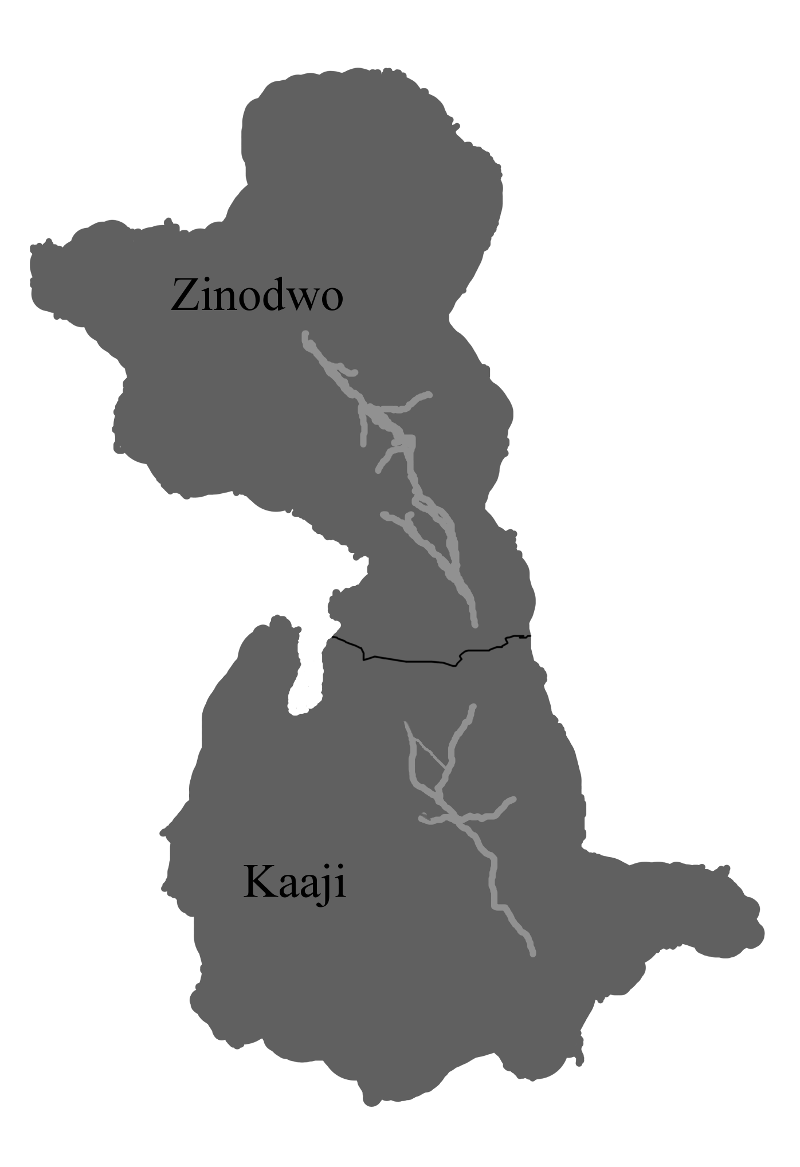
\includegraphics[width=4.5in]{Twizwa_map2.png}
\end{figure}
\clearpage

\section{Graft's}
I grew tired of looking at Pa\-co\-itz' map so I made my own using hints from the text. It's more accurate and way more informative, however, I did take some liberties.
\begin{figure}
\centering
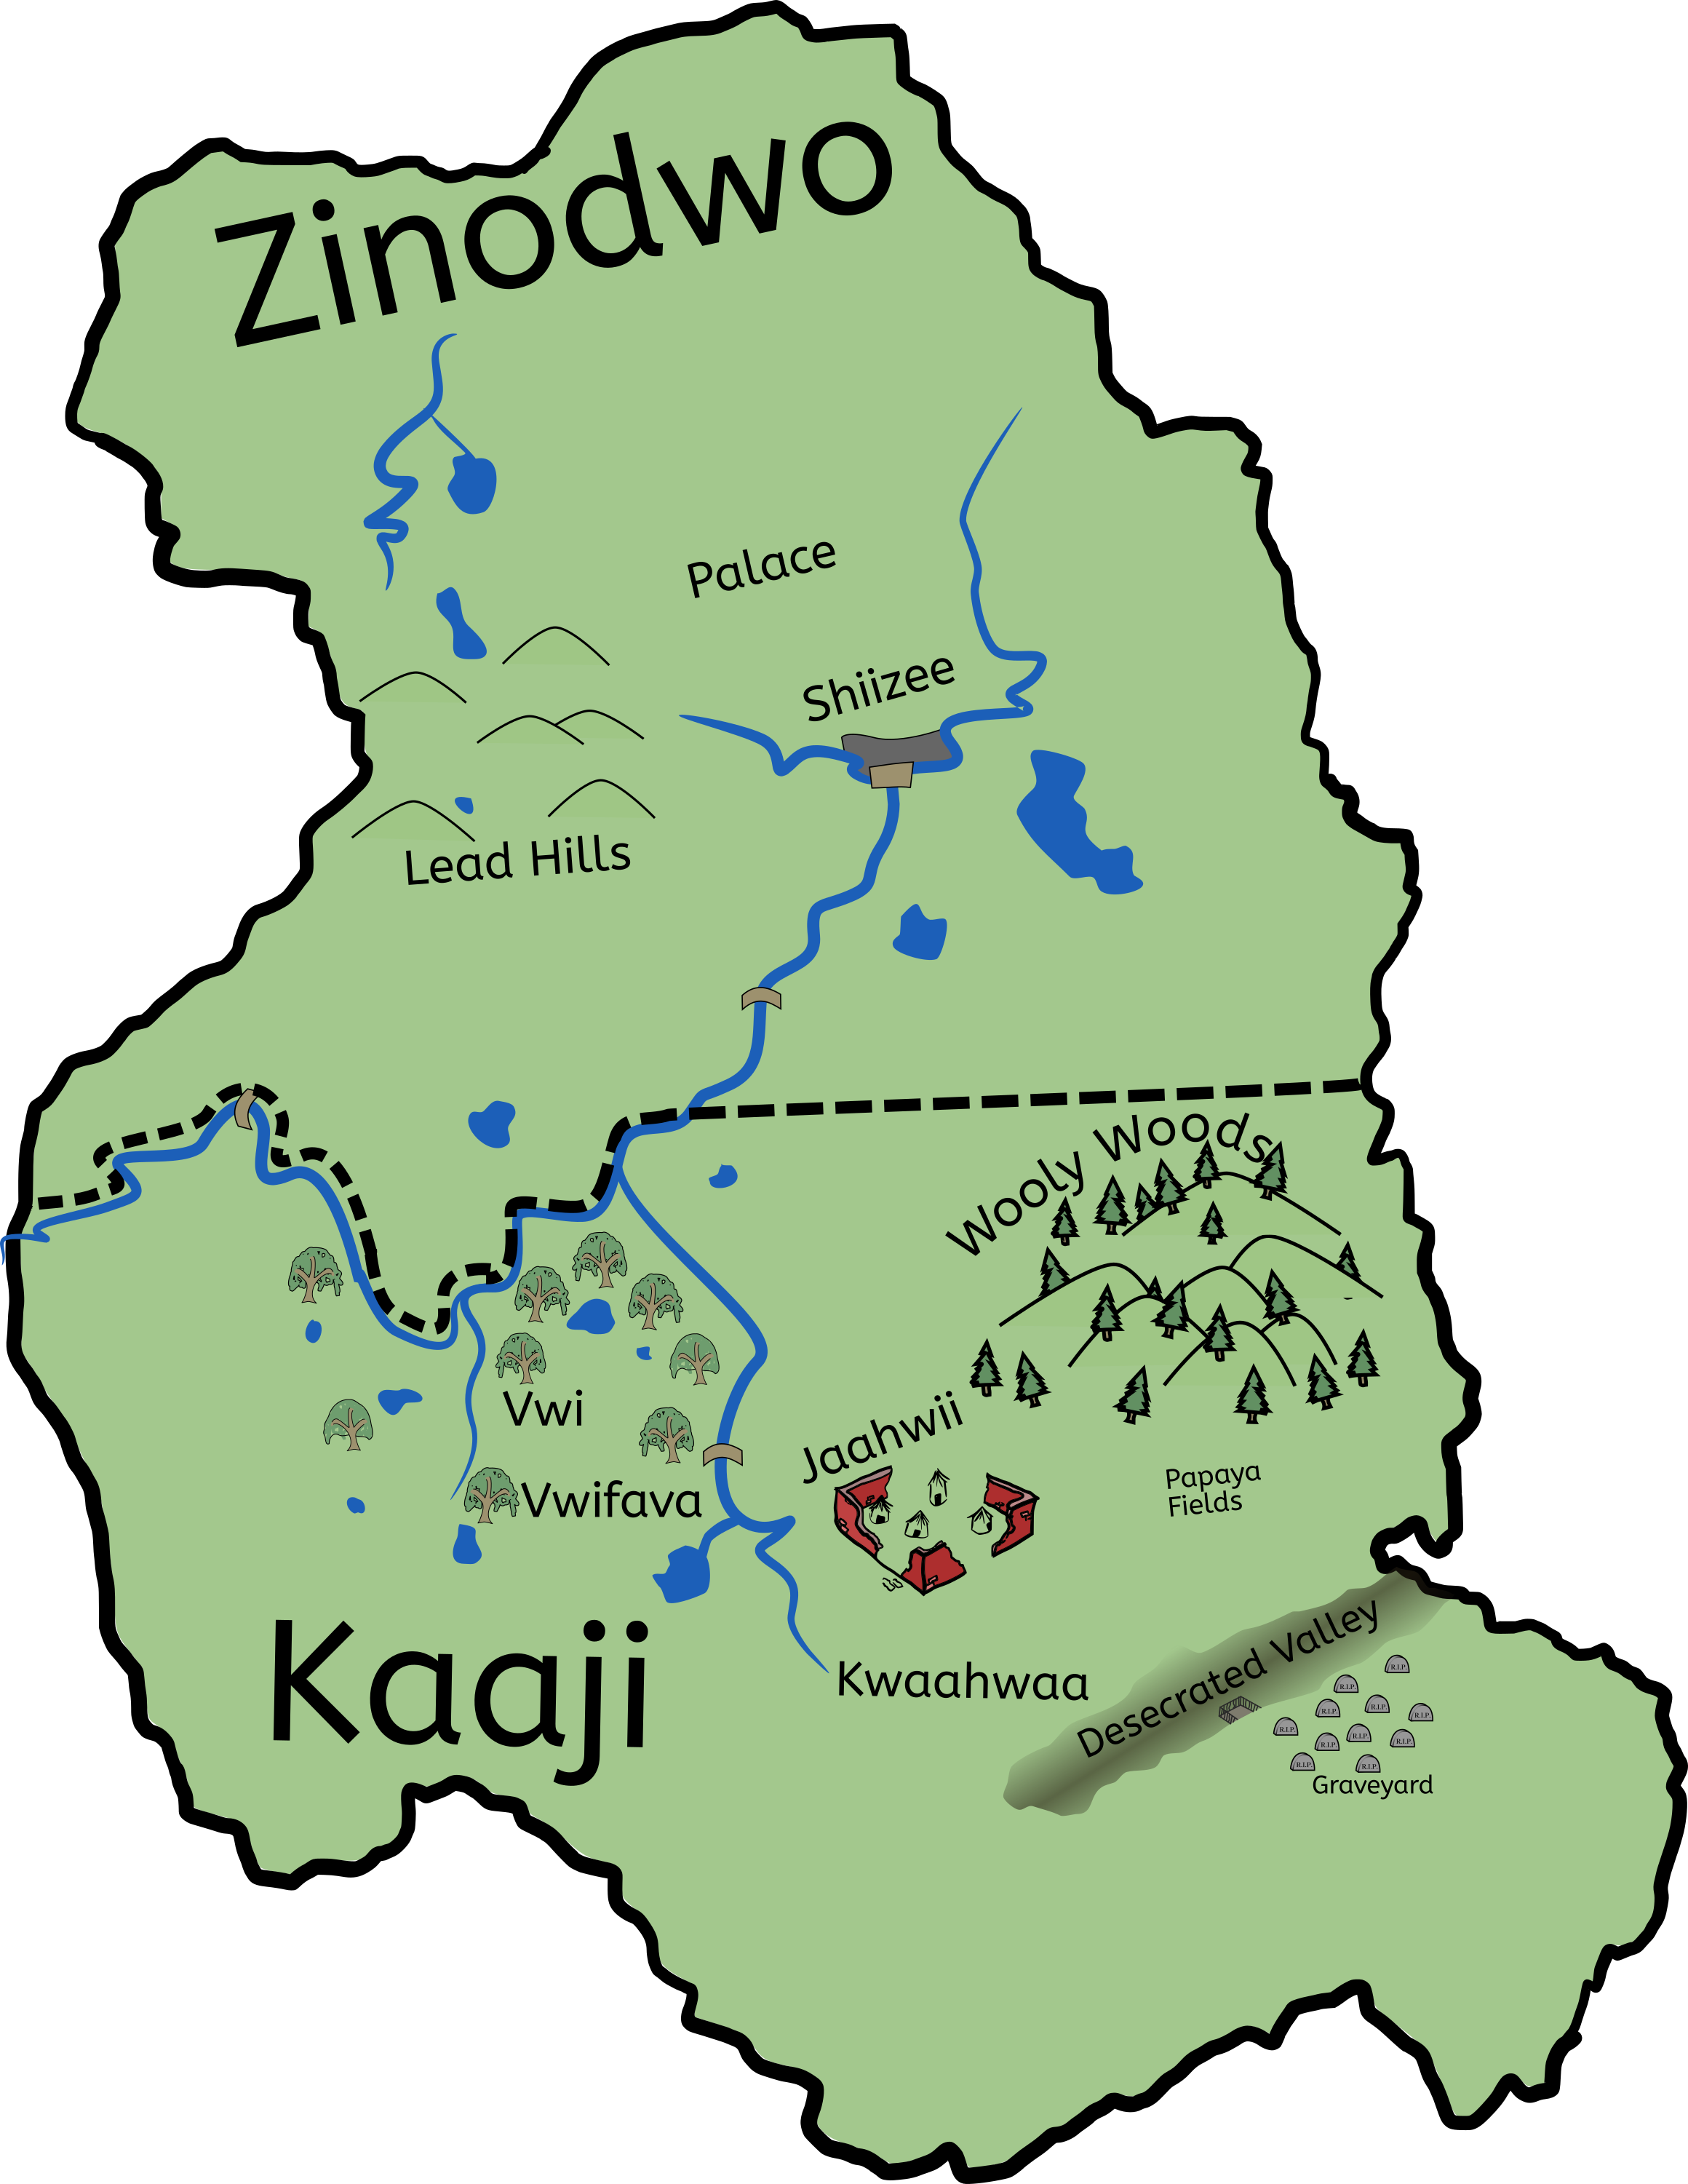
\includegraphics[width=4.0in]{map.png}
\end{figure}

\clearpage

\tableofcontents
\mainmatter
